\hypertarget{day-12---ux7f16ux5199ux65e5ux5fd7ux5217ux8868ux9875}{%
\subsection{Day 12 -
编写日志列表页}\label{day-12---ux7f16ux5199ux65e5ux5fd7ux5217ux8868ux9875}}

MVVM 模式不但可用于 Form
表单,在复杂的管理页面中也能大显身手。例如,分页显示 Blog
的功能,我们先把后端代码写出来:

在\texttt{apis.py}中定义一个\texttt{Page}类用于存储分页信息:

\begin{pythoncode}
class Page(object):

    def __init__(self, item_count, page_index=1, page_size=10):
        self.item_count = item_count
        self.page_size = page_size
        self.page_count = item_count // page_size + (1 if item_count % page_size > 0 else 0)
        if (item_count == 0) or (page_index > self.page_count):
            self.offset = 0
            self.limit = 0
            self.page_index = 1
        else:
            self.page_index = page_index
            self.offset = self.page_size * (page_index - 1)
            self.limit = self.page_size
        self.has_next = self.page_index < self.page_count
        self.has_previous = self.page_index > 1

    def __str__(self):
        return 'item_count: %s, page_count: %s, page_index: %s, page_size: %s, offset: %s, limit: %s' % (self.item_count, self.page_count, self.page_index, self.page_size, self.offset, self.limit)

    __repr__ = __str__
\end{pythoncode}

在\texttt{handlers.py}中实现 API:

\begin{pythoncode}
@get('/api/blogs')
def api_blogs(*, page='1'):
    page_index = get_page_index(page)
    num = yield from Blog.findNumber('count(id)')
    p = Page(num, page_index)
    if num == 0:
        return dict(page=p, blogs=())
    blogs = yield from Blog.findAll(orderBy='created_at desc', limit=(p.offset, p.limit))
    return dict(page=p, blogs=blogs)
\end{pythoncode}

管理页面:

\begin{pythoncode}
@get('/manage/blogs')
def manage_blogs(*, page='1'):
    return {
        '__template__': 'manage_blogs.html',
        'page_index': get_page_index(page)
    }
\end{pythoncode}

模板页面首先通过 API:\texttt{GET\ /api/blogs?page=?}拿到 Model:

\begin{pythoncode}
{
    "page": {
        "has_next": true,
        "page_index": 1,
        "page_count": 2,
        "has_previous": false,
        "item_count": 12
    },
    "blogs": [...]
}
\end{pythoncode}

然后,通过 Vue 初始化 MVVM:

\begin{pythoncode}
<script>
function initVM(data) {
    var vm = new Vue({
        el: '#vm',
        data: {
            blogs: data.blogs,
            page: data.page
        },
        methods: {
            edit_blog: function (blog) {
                location.assign('/manage/blogs/edit?id=' + blog.id);
            },
            delete_blog: function (blog) {
                if (confirm('确认要删除“' + blog.name + '”?删除后不可恢复!')) {
                    postJSON('/api/blogs/' + blog.id + '/delete', function (err, r) {
                        if (err) {
                            return alert(err.message || err.error || err);
                        }
                        refresh();
                    });
                }
            }
        }
    });
    $('#vm').show();
}
$(function() {
    getJSON('/api/blogs', {
        page: {{ page_index }}
    }, function (err, results) {
        if (err) {
            return fatal(err);
        }
        $('#loading').hide();
        initVM(results);
    });
});
</script>
\end{pythoncode}

View 的容器是\texttt{\#vm},包含一个
table,我们用\texttt{v-repeat}可以把 Model
的数组\texttt{blogs}直接变成多行的\texttt{\textless{}tr\textgreater{}}:

\begin{pythoncode}
<div id="vm" class="uk-width-1-1">
    <a href="/manage/blogs/create" class="uk-button uk-button-primary"><i class="uk-icon-plus"></i> 新日志</a>

    <table class="uk-table uk-table-hover">
        <thead>
            <tr>
                <th class="uk-width-5-10">标题 / 摘要</th>
                <th class="uk-width-2-10">作者</th>
                <th class="uk-width-2-10">创建时间</th>
                <th class="uk-width-1-10">操作</th>
            </tr>
        </thead>
        <tbody>
            <tr v-repeat="blog: blogs" >
                <td>
                    <a target="_blank" v-attr="href: '/blog/'+blog.id" v-text="blog.name"></a>
                </td>
                <td>
                    <a target="_blank" v-attr="href: '/user/'+blog.user_id" v-text="blog.user_name"></a>
                </td>
                <td>
                    <span v-text="blog.created_at.toDateTime()"></span>
                </td>
                <td>
                    <a href="#0" v-on="click: edit_blog(blog)"><i class="uk-icon-edit"></i>
                    <a href="#0" v-on="click: delete_blog(blog)"><i class="uk-icon-trash-o"></i>
                </td>
            </tr>
        </tbody>
    </table>

    <div v-component="pagination" v-with="page"></div>
</div>
\end{pythoncode}

往 Model 的\texttt{blogs}数组中增加一个 Blog 元素,table
就神奇地增加了一行;把\texttt{blogs}数组的某个元素删除,table
就神奇地减少了一行。所有复杂的 Model-View 的映射逻辑全部由 MVVM
框架完成,我们只需要在 HTML
中写上\texttt{v-repeat}指令,就什么都不用管了。

可以把\texttt{v-repeat="blog:\ blogs"}看成循环代码,所以,可以在一个\texttt{\textless{}tr\textgreater{}}内部引用循环变量\texttt{blog}。\texttt{v-text}和\texttt{v-attr}指令分别用于生成文本和
DOM 节点属性。

完整的 Blog 列表页如下:

 
 \begin{figure}[htp]
	\centering
	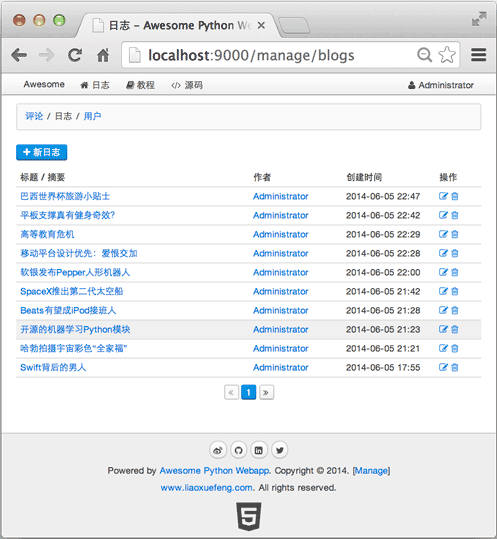
\includegraphics[width=0.6\linewidth]{fig/956084297542656.png}
\end{figure}


\hypertarget{ux53c2ux8003ux6e90ux7801}{%
\subsubsection{参考源码}\label{ux53c2ux8003ux6e90ux7801}}

\href{https://github.com/michaelliao/awesome-python3-webapp/tree/day-12}{day-12}

